\documentclass[tikz,border=3mm]{standalone}
\usetikzlibrary{calc} % Used for coordinate calculations

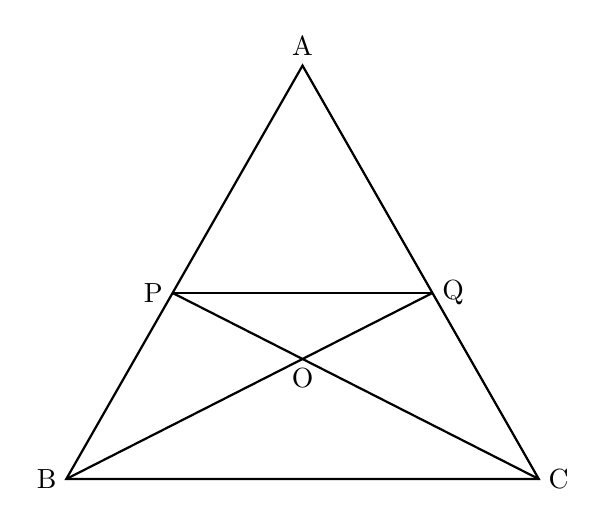
\begin{tikzpicture}[scale=1.5]
    % Define the vertices of the main triangle ABC
    % A is at the top, B at bottom-left, C at bottom-right
    \coordinate (B) at (0,0);
    \coordinate (C) at (4,0);
    \coordinate (A) at (2,3.5);

    % Define points P and Q
    % P is on AB, Q is on AC. Visually they appear to be slightly below the midpoint.
    % Using barycentric coordinates: 0.55 distance from A to vertices.
    \coordinate (P) at ($(A)!0.55!(B)$);
    \coordinate (Q) at ($(A)!0.55!(C)$);

    % Define point O as the intersection of diagonals BQ and CP
    \coordinate (O) at (intersection of B--Q and C--P);

    % Draw the main Triangle ABC
    \draw[thick] (A) -- (B) -- (C) -- cycle;

    % Draw the horizontal segment PQ
    \draw[thick] (P) -- (Q);

    % Draw the intersecting segments BQ and CP
    \draw[thick] (B) -- (Q);
    \draw[thick] (C) -- (P);

    % Add Labels
    \node[above] at (A) {A};
    \node[left] at (B) {B};
    \node[right] at (C) {C};
    \node[left] at (P) {P};
    \node[right] at (Q) {Q};
    \node[below] at (O) {O};

\end{tikzpicture}